\section{Introduction}
\label{sec:introduction}

Driven by its clean nature and reliable supply, wind power has become an important energy source for modern power systems. Accurate wind speed and direction forecasting is essential for grid dispatch, resource allocation, and wind-energy utilization \cite{Hanifi2020CriticalReviewWindPowerForecasting,Jung2014CurrentStatusWindSpeedPowerForecasting}. However, existing methods typically process different wind speed and direction using a single, unified approach. This approach overlooks a critical physical reality: wind speed and wind direction possess fundamentally distinct cross-turbine structures and mathematical properties \cite{Chen2014WindPowerForecastsGaussianProcesses,Dolatabadi2022DeepSpatialTemporal2DCNNBLSTM}.

As illustrated in Fig.~\ref{fig:data_properties}, wind speed and wind direction show different modeling properties. First, wind speed exhibits a strong shared property: because the turbines are driven by similar weather patterns, their trajectories usually follow comparable trends. Therefore, effective wind-speed modeling should leverage these shared dynamics.


\begin{figure}[!t]
	\centering
	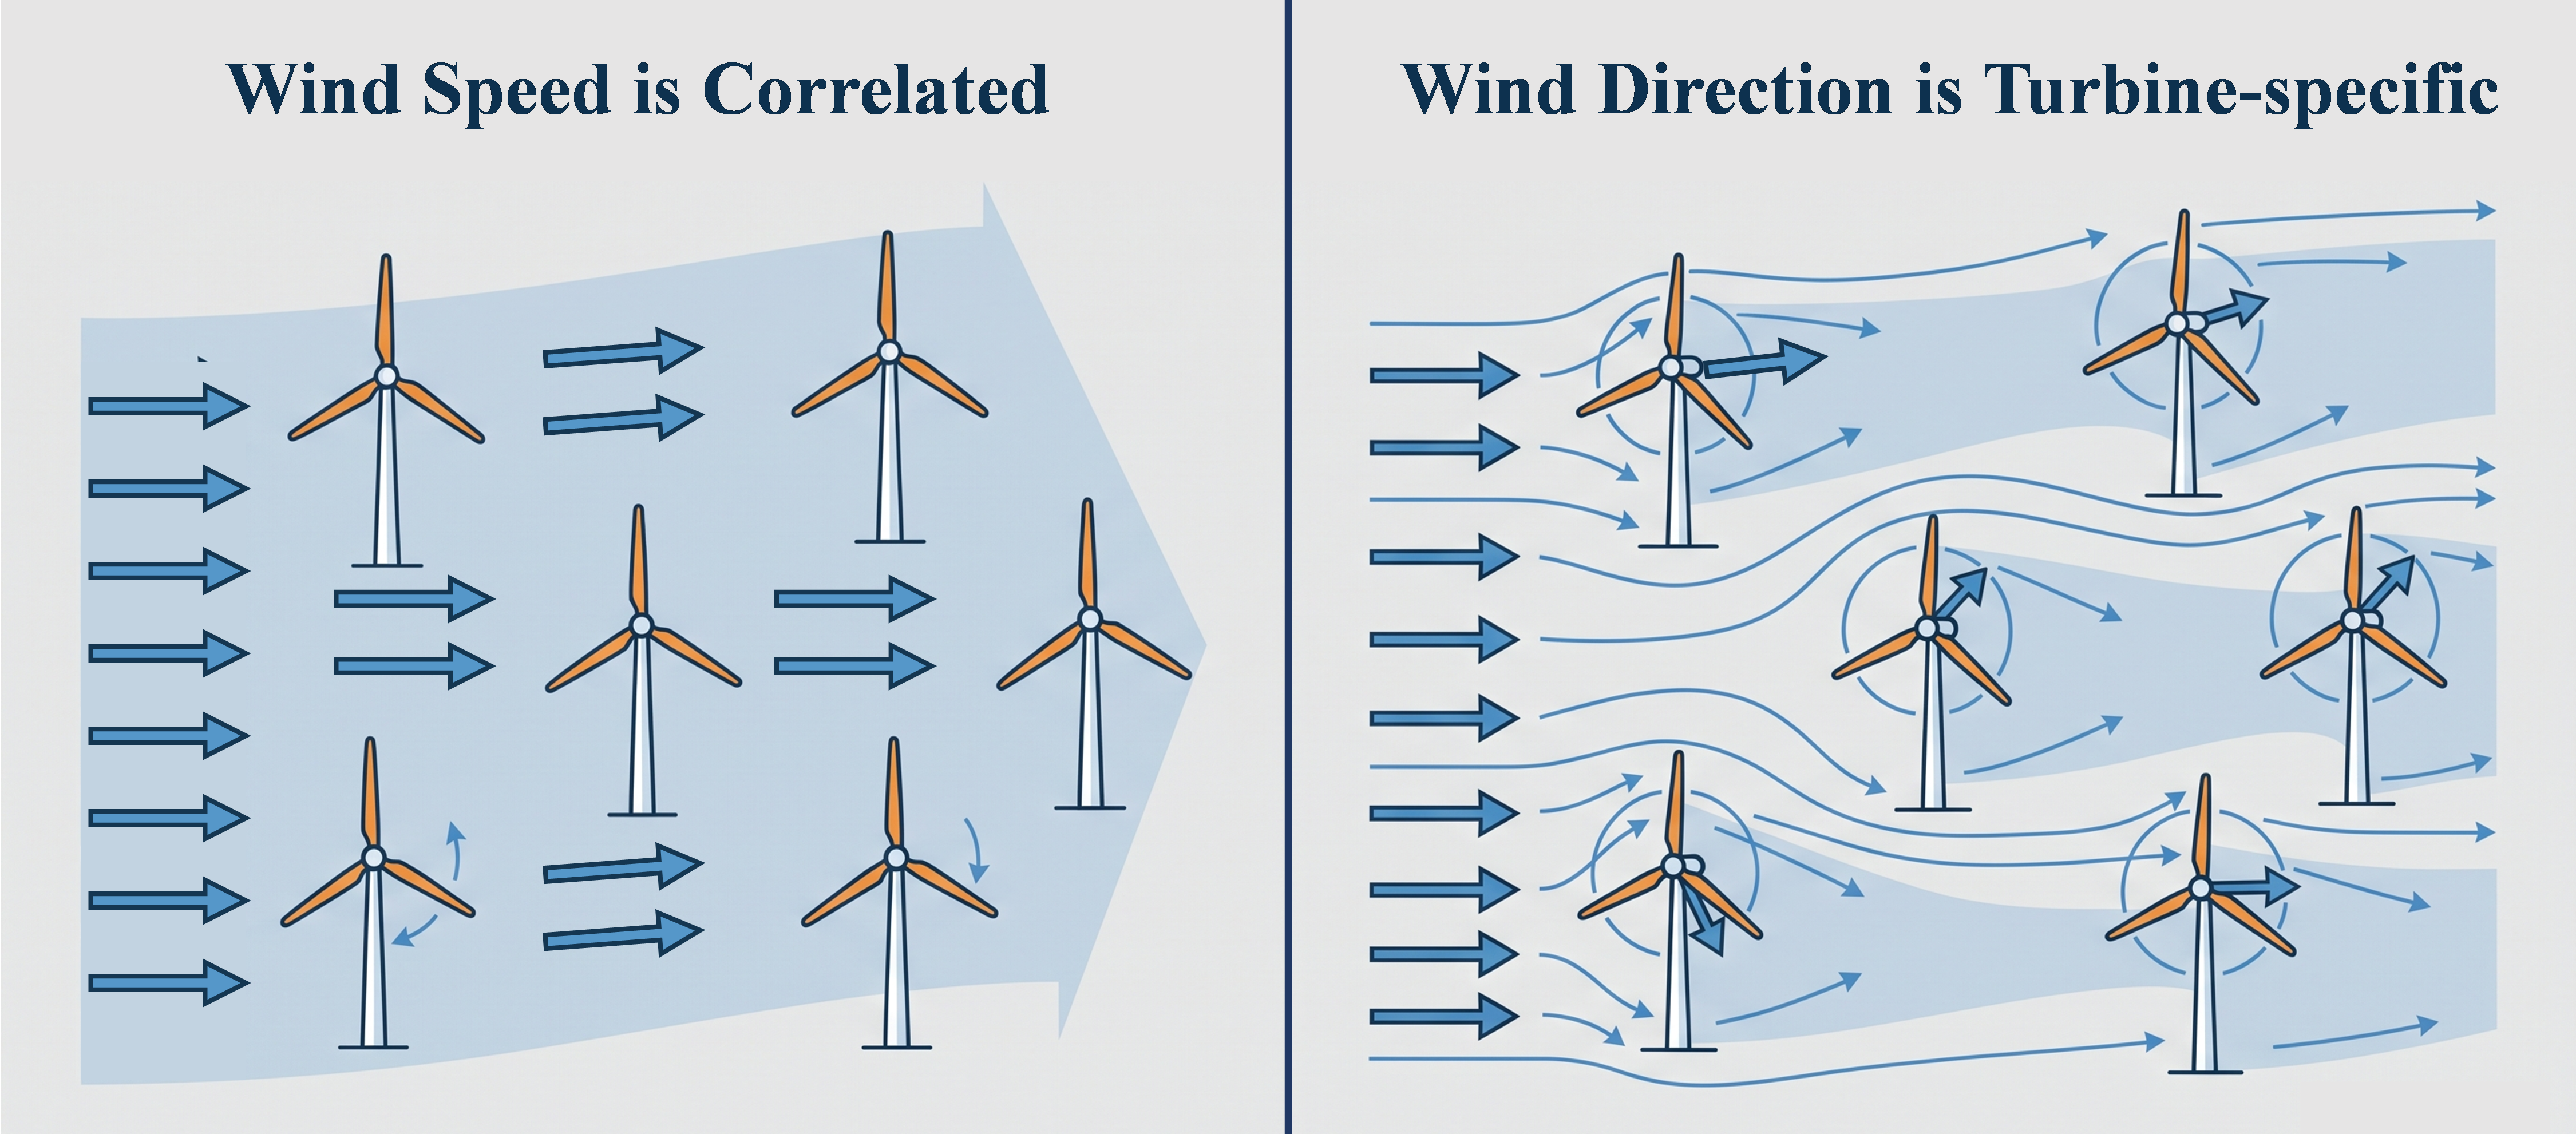
\includegraphics[width=0.48\textwidth]{figures/figure1.png}
	\caption{Conceptual contrast between cross-turbine wind-speed correlation and turbine-specific wind-direction variation.}
	\label{fig:data_properties}
\end{figure}

Second, wind direction presents different challenges. On the one hand, interactions among turbine spatial locations, wake effects, and local flow fields cause different units to exhibit distinct dominant directions and variation ranges. On the other hand, raw wind direction is usually recorded as a one-dimensional angle, which is discontinuous at the periodic boundary. For instance, $0^\circ$ and $360^\circ$ physically represent the same direction, and $359^\circ$ and $1^\circ$ differ by only $2^\circ$. If treated as a regular scalar, the model may misinterpret the latter as a massive $358^\circ$ separation. This misrepresentation turns physically continuous transitions into abrupt numerical jumps. Therefore, wind direction forecasting requires representations and error metrics that respect periodic continuity.

Based on the above observations, this paper focuses on the sharing property of wind speed and the periodic nature of wind direction, and further addresses two research questions(RQ):

\textbf{RQ1:}
How can we exploit the shared wind-speed dynamics among multiple turbines?

\textbf{RQ2:}
How can we preserve boundary continuity in wind-direction signals?

Driven by this motivation, we conduct an in-depth exploration of the two research questions detailed below.

\subsection{Wind Speed Forecasting}
\label{subsec:speed_sharing_intro}

Multiple turbines are affected by similar weather processes and large-scale wind fields, but local terrain and wake effects still produce turbine-level deviations. Channel-independent methods preserve these differences but repeatedly relearn common variations, whereas fully correlated methods may mix common and local dynamics. We therefore extract a shared wind field and model turbine-specific residuals separately.

Fig.~\ref{fig:speed_multiscale_similarity} further shows that representative turbines exhibit similar dominant frequency components and wavelet energy patterns, supporting the existence of shared multi-scale wind-speed dynamics across turbines.

\begin{figure}[!t]
\centering
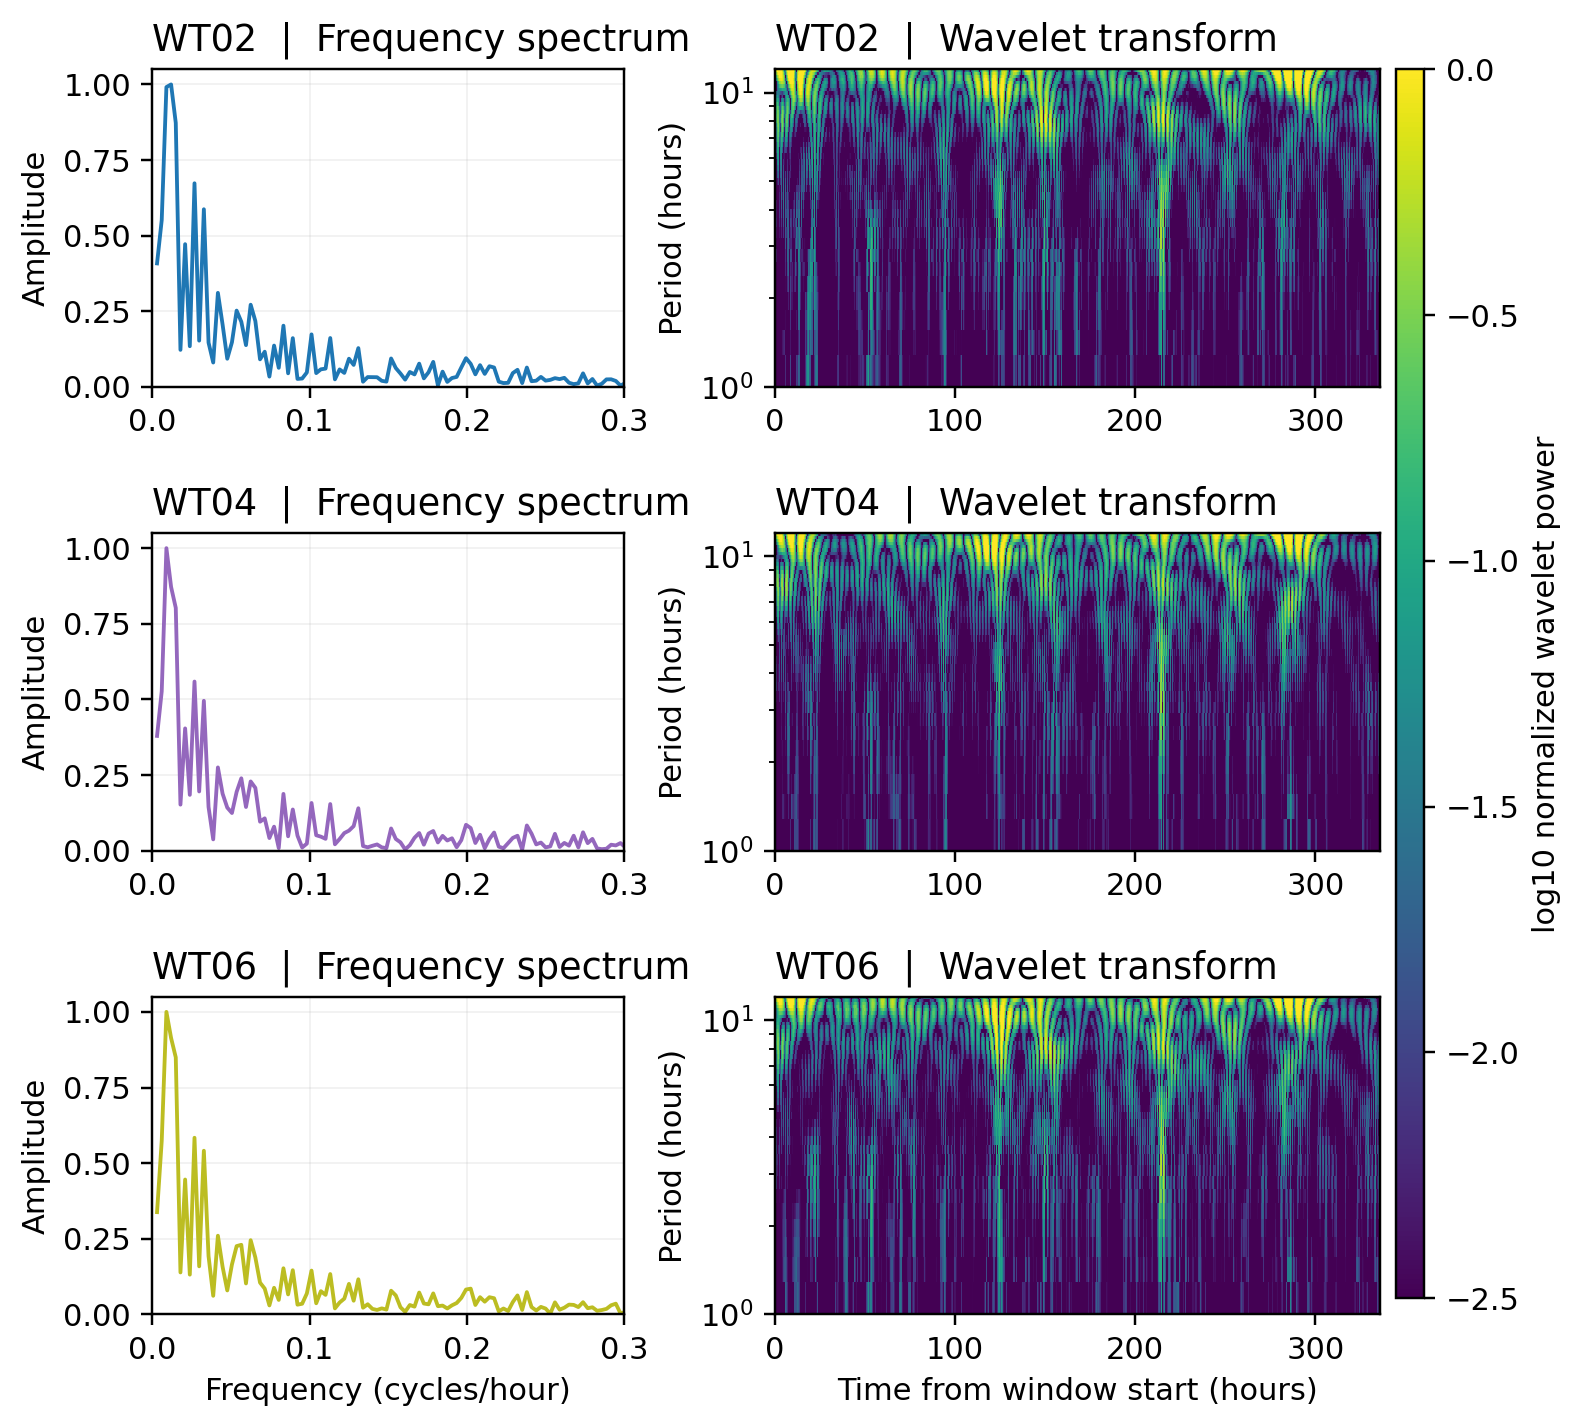
\includegraphics[width=0.48\textwidth]{figures/figure2.png}
\caption{Frequency-spectrum and wavelet-transform comparison of representative turbine wind-speed sequences. Similar dominant frequency components and wavelet energy patterns support the shared multi-scale dynamics of wind speed across turbines.}
\label{fig:speed_multiscale_similarity}
\end{figure}

After extracting the common wind field, we introduce a Phase representation. By aligning observations at similar evolutionary stages, this approach effectively captures periodic wind dynamics and mitigates distribution drift across time blocks.

\subsection{Wind Direction Forecasting}
\label{subsec:direction_2d_intro}

Wind speed and wind direction have different cross-turbine structures. The interaction among turbine locations, wakes, and local flow fields causes different units to present distinct dominant directions and turning patterns, so wind direction should not be collapsed into a common representation in the same way as wind speed. Fig.~\ref{fig:direction_specificity} (a) shows that the dominant directions and directional concentration levels of different turbines are not consistent. Fig.~\ref{fig:direction_specificity} (b) reveals that about 51\% of turbine pairs have an average angular distance of no less than $90^\circ$, indicating that cross-turbine directional differences are not caused by a few outliers. Fig.~\ref{fig:direction_specificity} (c) further displays the difference structure among 24 turbines using a pairwise angular distance matrix, where high and low angular distances alternate across regions, demonstrating that wind-direction relationships exhibit strong turbine-level dependence. Therefore, wind-direction modeling needs to preserve turbine-specific directional information.

\begin{figure}[!t]
\centering

\includegraphics[width=0.48\textwidth]{figures/all_24_turbines_direction_difference_summary.png}
\caption{Turbine-specific wind direction distributions and all-pair angular differences among 24 turbines.}
\label{fig:direction_specificity}
\end{figure}

In addition, wind direction is not a regular one-dimensional scalar because its numerical boundary is physically connected. Wind direction satisfies

\begin{equation}
\theta \equiv \theta+360^\circ.
\end{equation}

Direct scalar regression breaks this equivalence near the boundary and may distort distances, local variations, and error gradients. Thus, wind direction forecasting must preserve boundary continuity from the input representation, rather than merely correcting angles after prediction. To this end, this paper maps the one-dimensional direction angle of each turbine into a two-dimensional sine-cosine unit-vector representation:

\begin{equation}
\mathbf{u}_{t,n} = [\cos(\theta_{t,n}), \sin(\theta_{t,n})].
\end{equation}

This mapping keeps boundary-adjacent directions close to each other in the representation space and provides unified coordinates for subsequent forecasting and error calculation. On this basis, the model performs predictions in the two-dimensional direction space, uses direction-vector loss and vector-consistency loss to constrain the prediction results, and then restores the predicted components to angles:

\begin{equation}
\hat{\theta}_{t,n} = \operatorname{atan2} \left( \hat{u}^{\sin}_{t,n}, \hat{u}^{\cos}_{t,n} \right)
\end{equation}

For wind-direction forecasting, we segment the two-dimensional direction sequence of each turbine into patches and extract local temporal patterns using shared Patch Attention. Specifically, the sine-cosine representation resolves the boundary discontinuity by defining continuous directional coordinates and distance metrics, while the patch strategy structures the historical temporal sequences. Because dominant directions and turning patterns vary significantly across units, the wind-direction branch processes inputs and outputs on an individual turbine basis. However, since local temporal dynamics often contain transferable structures, all turbines share the same patch-attention module. This architecture prevents the inappropriate compression of distinct wind directions into a single global state while enabling shared temporal modeling within a physically consistent two-dimensional representation space.

\subsection{WindFormer Framework}

Based on these issues, this paper constructs WindFormer as a common-speed and direction-vector learning framework. For the wind-speed branch, WindFormer first extracts common wind-field dynamics from the wind speeds of multiple turbines through learnable weighted aggregation, treating the independent variation of each turbine as a local residual. Subsequently, the common wind field is modeled via attention using Phase as the basic unit, while local residuals are refined by lightweight MLPs. For the wind-direction branch, WindFormer first converts each one-dimensional direction angle into sine-cosine components to eliminate boundary discontinuities and then extracts directional variation patterns through turbine-wise Patch sequences and shared Patch Attention. The two branches remain structurally decoupled and are trained jointly through a unified loss.

The main contributions of this paper are as follows:

\begin{itemize}
	\item \textbf{In terms of wind-speed modeling, we propose a common-wind-field modeling strategy.} This method first extracts cross-turbine shared wind-field dynamics and then models the independent local variations of each turbine. To represent recurring variation processes within the common wind field, we introduce Phase representation to align similar cross-period processes.
    \item \textbf{In terms of wind-direction modeling, we propose a two-dimensional unit-vector representation strategy for multi-turbine wind direction forecasting.} Because raw wind direction is a one-dimensional angle with boundary discontinuity, we retain turbine-wise wind direction sequences and adopt sine-cosine components to describe distribution differences and directional variation patterns more faithfully.
    \item \textbf{We develop and comprehensively evaluate a structure-aware dual-branch forecasting algorithm.} WindFormer jointly predicts wind speed and wind direction through task-specific branches and a unified training objective. Standard forecasting, robustness tests, and sparse-deployment zero-shot experiments further verify its accuracy, stability, and cross-turbine generalization.
\end{itemize}

\section{Related Work}
\label{sec:related_work}

\subsection{Spatial Relationships in Multi-Turbine Wind Power Forecasting}

Existing deep learning studies usually improve wind forecasting by modeling spatial relationships among turbines. Graph-based and convolutional recurrent models encode turbine topology, neighborhood influence, multi-scale spatial dependence, or local and long-range interactions into the forecasting process \cite{Song2023ShortTermForecastingGraphConvolutionWindPower,Zhang2019LSTMNeighborhoodGatesCausalityWindSpeed,Wu2024MixFormerHierarchicalContextWindSpeed}. To handle condition-dependent relationships, later studies further introduce channel-aware dependence and temporal lead-lag structures \cite{Zhao2024RethinkingChannelDependenceLeadingIndicators,Zhu2024GGNetTemporalLeadLagCorrelations}. These methods show that cross-turbine information is useful for short-term wind forecasting.

Generic multivariate time-series models also provide useful designs for organizing turbine variables. PatchTST reduces cross-channel interference through channel-independent temporal modeling \cite{Nie2023PatchTST}, TimesNet converts temporal variations into two-dimensional period structures \cite{Wu2023TimesNetTemporal2DVariationModeling}, iTransformer learns dependencies along the variable dimension \cite{Liu2024iTransformer}, and MSGNet enhances multi-scale cross-sequence interaction \cite{Cai2024MSGNetLearningMultiScaleInterSeriesCorrelations}. MST-Net further discusses the combination of channel-independent and spatially correlated modeling for short-term wind resource forecasting \cite{Lou2026MSTNet}. More recently, an Information Sciences study further explores a global-local dual-branch design and pyramid patch interaction for multivariate forecasting \cite{Zhou2026GLPTGlobalLocalPyramidTransformer}.

However, most existing methods regard cross-turbine relationships as a single interaction pattern to be learned. They seldom separate the common wind-speed field shared by multiple turbines from turbine-specific residual variations. This distinction is important because wind speeds in the same wind farm often share dominant meteorological trends, while local terrain, wake effects, and turbine positions still introduce individual deviations.

\subsection{Wind Direction Forecasting and Two-Dimensional Representation}

Wind direction forecasting has been studied together with wind speed prediction, yaw-state modeling, and short-term directional change prediction. Representative works include ARMA-based joint wind speed and direction forecasting \cite{Erdem2011ARMATupleWindSpeedDirection}, yaw-error prediction based on wind-direction changes \cite{Ouyang2017PredictiveYawError}, and two-phase deep models designed for short-term wind-direction sequences \cite{Tang2021TwoPhaseWindDirection}.

Unlike wind speed, raw wind direction is a one-dimensional angle with boundary discontinuity. Sine-cosine representations provide a natural way to embed direction angles into a continuous two-dimensional space \cite{Erdem2011ARMATupleWindSpeedDirection,Ouyang2017PredictiveYawError}. Nevertheless, existing studies mainly focus on single direction sequences or general speed-direction joint prediction. Systematic modeling of multi-turbine directional heterogeneity under periodic-boundary constraints remains insufficiently explored.
